\documentclass[a4paper, 10pt]{article}

\usepackage{vmargin}

\setmarginsrb{2cm}{0cm}{2cm}{0,2cm}{1cm}{1,5cm}{1cm}{1,5cm}
%1 est la marge gauche
%2 est la marge en haut
%3 est la marge droite
%4 est la marge en bas
%5 fixe la hauteur de l'entête
%6 fixe la distance entre l'entête et le texte
%7 fixe la hauteur du pied de page
%8 fixe la distance entre le texte et le pied de page
%------------------------------Packages généraux------------------------------

\usepackage[english]{babel}
\usepackage[T1]{fontenc}
\usepackage{ae}
\usepackage[utf8]{inputenc}
\usepackage{scrextend}
\usepackage{hyperref}

%-------------------------Mathématiques------------------------------
\usepackage{amsmath}
\usepackage{amssymb}
\usepackage{amsthm}
\usepackage{amsfonts}
\usepackage{eucal}
\newcommand\independent{\protect\mathpalette{\protect\independenT}{\perp}}
\def\independenT#1#2{\mathrel{\rlap{$#1#2$}\mkern2mu{#1#2}}}
%-----------------------Codes et algorithmes--------------------------
\usepackage{algorithm}
\usepackage{algorithmic}
\usepackage{clrscode3e}

%------------------------------Graphics------------------------------

\usepackage{graphicx}
\usepackage{fancyhdr}
\usepackage{fancybox}
\usepackage{color}
\usepackage{pgf, tikz}
\usetikzlibrary{arrows, automata}
%\usepackage{slashbox}
%------------------------------Syntaxe------------------------------

\usepackage{listings}
\lstloadlanguages{Matlab}

\def\refmark#1{\hbox{$^{\ref{#1}}$}}
\DeclareSymbolFont{cmmathcal}{OMS}{cmsy}{m}{n} %Mathcal correcte
\DeclareSymbolFontAlphabet{\mathcal}{cmmathcal}

%------------------------------Inclure code MatLab------------------------------

\usepackage{listings}
\newcommand*\styleC{\fontsize{9}{10pt}\usefont{T1}{ptm}{m}{n}\selectfont }
\newcommand*\styleD{\fontsize{9}{10pt}\usefont{OT1}{pag}{m}{n}\selectfont }

%------------------Sub-sections--------%
\usepackage{titlesec}
\usepackage{hyperref}

\renewcommand\thesubsubsection{\alph{subsubsection}}

\titleclass{\subsubsubsection}{straight}[\subsubsection]

\newcounter{subsubsubsection}[subsubsection]
\renewcommand\thesubsubsubsection{\thesubsubsection.\arabic{subsubsubsection}}

\titleformat{\subsubsubsection}
  {\normalfont\normalsize\bfseries}{\thesubsubsubsection}{1em}{}
\titlespacing*{\subsubsubsection}
{0pt}{3.25ex plus 1ex minus .2ex}{1.5ex plus .2ex}


\makeatletter
% on fixe le langage utilisé
\lstset{language=matlab}
\edef\Motscle{emph={\lst@keywords}}
\expandafter\lstset\expandafter{%
  \Motscle}
\makeatother


\definecolor{Ggris}{rgb}{0.45,0.48,0.45}

\lstset{emphstyle=\rmfamily\color{blue}, % les mots réservés de matlab en bleu
basicstyle=\styleC,
keywordstyle=\ttfamily,
commentstyle=\color{Ggris}\styleD, % commentaire en gris
numberstyle=\tiny\color{red},
numbers=left,
numbersep=10pt,
lineskip=0.7pt,
showstringspaces=false}
%  % inclure le fichier source
\newcommand{\FSource}[1]{%
\lstinputlisting[texcl=true]{#1}
}

\usepackage[section]{placeins}

\let\cleardoublepage\clearpage

\usepackage{hyperref}
               
 \hypersetup{
    colorlinks = true,
    linkcolor=black,
    urlcolor = black
    }
%------------------------------Début du document------------------------------
\begin{document}
%------------------------------Page de garde------------------------------


  % \frontmatter
  %\tableofcontents
   \setcounter{page}{1}
   %%%%%%%%% TP 4 %%%%%%%%%%%
   \section{Reasoning under uncertainty I (08/11/2018)}
   \subsection{Objectives}
      At the end of this repetition you should be able to:
      \begin{itemize}
          \item Apply Bayes rules, independence and marginalisation appropriately to compute probabilities
      \end{itemize}
\subsection{Exercises}
   \subsubsection{$\approx 10$ min}
   Let two events A, B of the probability space $\Omega$; Is it possible to get $P(A)=0.4$, $P(B)=0.3$, and
    $P(A\vee B)=0.5$? If so, what range of probabilities would be possible for $A\wedge B$?
    \subsubsection{$\approx 15$ min}
    Given the probability table of Figure \ref{fig:p_table} compute the following probabilities:
    \begin{enumerate}
        \item P(toothache)
        \item P(cavity)
        \item P(toothache | cavity)
        \item P(cavity | toothache $\vee$ catch)
    \end{enumerate}
    \begin{figure}[H]
        \centering
        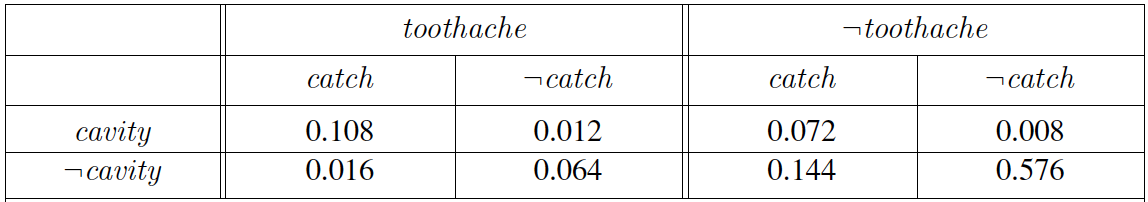
\includegraphics[width=1.\textwidth]{figures/proba_table.png}
        \caption{Probablity Table of Toothache and Cavity}
        \label{fig:p_table}
    \end{figure}
    \subsubsection{$\approx 10$ min}
    After your yearly checkup, the doctor has bad news and good news. The bad news
is that you tested positive for a serious disease and that the test is 99\% accurate (i.e., the
probability of testing positive when you do have the disease is 0.99, as is the probability of
testing negative when you don’t have the disease). The good news is that this is a rare disease,
striking only 1 in 10,000 people of your age. Why is it good news that the disease is rare?
What are the chances that you actually have the disease?

   \subsection{Supplementary material}
   \url{https://www.youtube.com/watch?v=x-2uVNze56s}
   
 
   
   
\end{document}
